\section{PGP}
\subsection{PGP}
\begin{frame}
    \frametitle{\color{white}PGP}
    \begin{block}{Qu'est-ce que PGP ?}
      \begin{itemize}
       \item Logiciel créé par Phil Zimmermann en 1991.
         \item Pretty Good Privacy = Assez bonne confidentialité
       \end{itemize} 
    \end{block}
    \begin{block}{Pourquoi ?}
      \begin{itemize}
         \item Permettre l'utilisation de la cryptographie pour le grand public
         \item Chiffrer, déchiffrer, signer et vérifier des données. 
         \item Échanger des emails de manière sûre.
       \end{itemize} 
    \end{block}
\end{frame}
\begin{frame}
    \frametitle{\color{white}PGP et la cryptographie hybride}
    \begin{block}{Comment ?}
      \begin{itemize}
         \item Utilisation de cryptographie hybride = symétrique + asymétrique
         \item Les données sont chiffrées ou déchiffrées par clef symétrique.
   \item Les clefs symétriques utilisées sont chiffrées ou déchiffrées par les clefs asymétriques des utilisateurs.
         \item Un utilisateur doit donc posséder:
    \begin{itemize}
      \item Sa propre paire de clefs asymétriques (privée et public).
      \begin{itemize}
        \item La clef privée sert à signer et déchiffrer.
        \item La clef publique sert à chiffrer et vérifier.
      \end{itemize}
      \item Les clefs publiques des personnes avec qui il souhaite communiquer.
      \begin{itemize}
        \item Pour chiffrer des données qui leur sont destinées.
        \item Pour vérifier des données qu'ils ont signées.
      \end{itemize}
    \end{itemize}
   \item Les utilisateurs doivent donc partager leur clef publique avec leurs contacts.
       \end{itemize} 
    \end{block}
\end{frame}

\begin{frame}
    \frametitle{\color{white}PGP - Les Clefs}
    \begin{block}{Qu'est-ce qu’une clef PGP ?}
      \begin{itemize}
    \item Une clef asymétrique privée ou publique.
    \item Une date de création.
    \item Une empreinte ( = le haché de : la clef + la date de création)
    \item Un utilisateur (nom et adresse email).
    \item Une auto signature (faite par cette même clef).
    \item Un niveau de validité.
    \item Un niveau de confiance.
       \end{itemize} 
    \end{block}
\end{frame}

\begin{frame}
  \frametitle{\color{white}PGP - Le modèle de confiance}
    \begin{block}{Le concept de toile de confiance}
      \begin{itemize}
    \item Les amis de mes amis sont mes amis.
    \item Certification de clef :
      \begin{itemize}
       \item La personne qui détient cette clef est-elle bien celle qu'elle prétend être ?
       \item Si oui, on peut la certifier -> la clef est alors complètement valide.
      \end{itemize}
    \item Attribution d'un niveau de confiance :
      \begin{itemize}
       \item Cette personne vérifie-t-elle correctement les clefs qu'elle certifie ?
       \item Peut-on considérer les clefs qu'elle a certifiées comme valides ? À quel niveau ?
       \item La confiance d'une clef impacte les autres clefs signées par celle-ci.
      \end{itemize}   
       \end{itemize} 
    \end{block}
\end{frame}
\begin{frame}
  \frametitle{\color{white}PGP - Le modèle de confiance}
    \begin{block}{Validité non définie}
      Alice n'a pas attribué de confiance aux trois clefs qu'elle a certifiées.\\
      La clé non certifiée par Alice n'est donc pas valide.
    \end{block}
    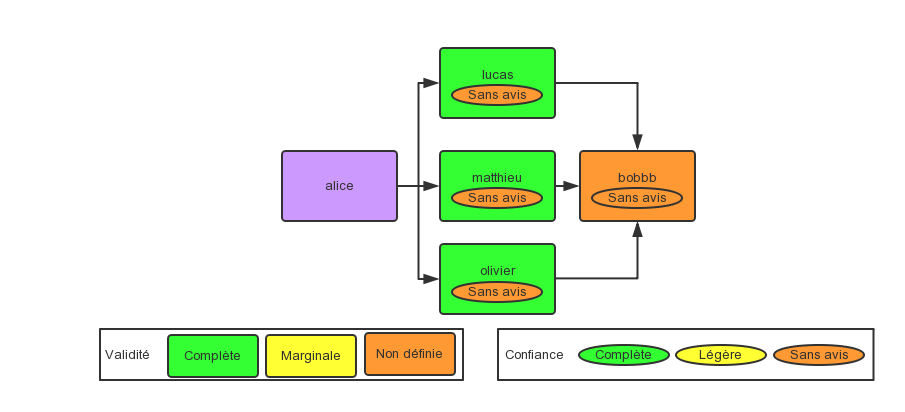
\includegraphics[scale=0.3]{tdcdemoUndefined.png}
\end{frame}
\begin{frame}
  \frametitle{\color{white}PGP - Le modèle de confiance}
    \begin{block}{Validité Marginal}
      Une ou deux clefs certifiées par Alice avec une confiance légère 
      induisent une validité marginale sur la clé non certifiée par Alice.
    \end{block}
    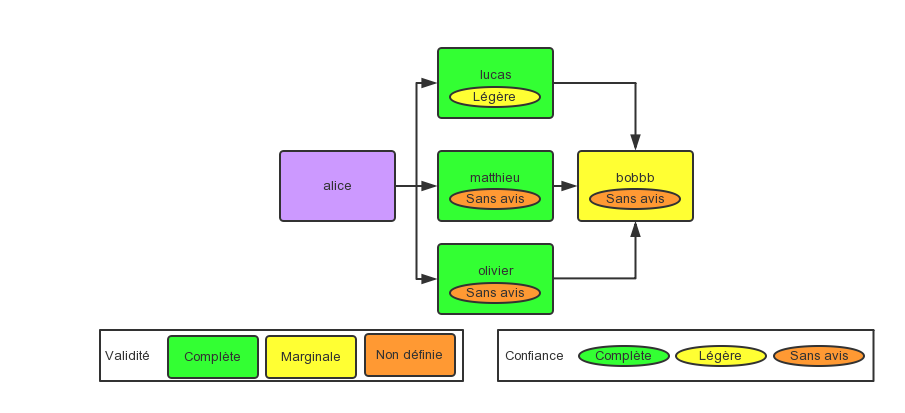
\includegraphics[scale=0.3]{tdcdemoMarginal.png}
\end{frame}
\begin{frame}
  \frametitle{\color{white}PGP - Le modèle de confiance}
    \begin{block}{Validité Complète}
      Trois clefs ou plus certifiés par Alice avec une confiance légère
      induite une validité complète sur la clé non certifiée par Alice.
    \end{block}
    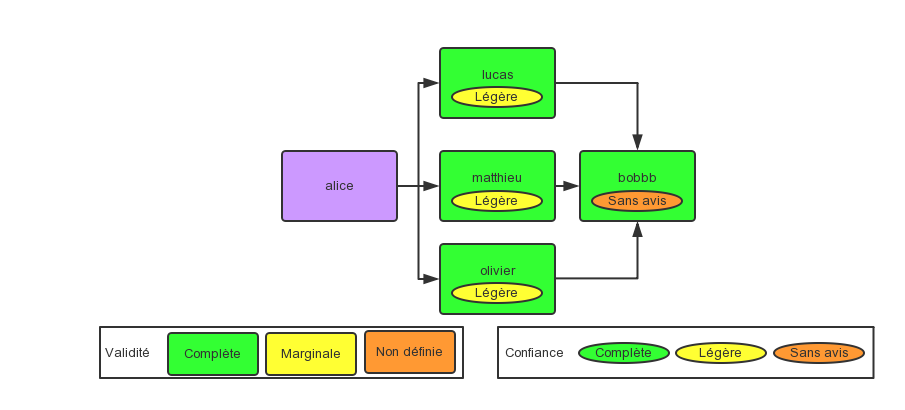
\includegraphics[scale=0.3]{tdcdemoComplete1.png}
\end{frame}
\begin{frame}
  \frametitle{\color{white}PGP - Le modèle de confiance}
    \begin{block}{Validité Complète}
      Une clef certifiée par Alice avec une confiance complète
      suffit à propager une validité complète sur la clé non certifiée par Alice.
    \end{block}
    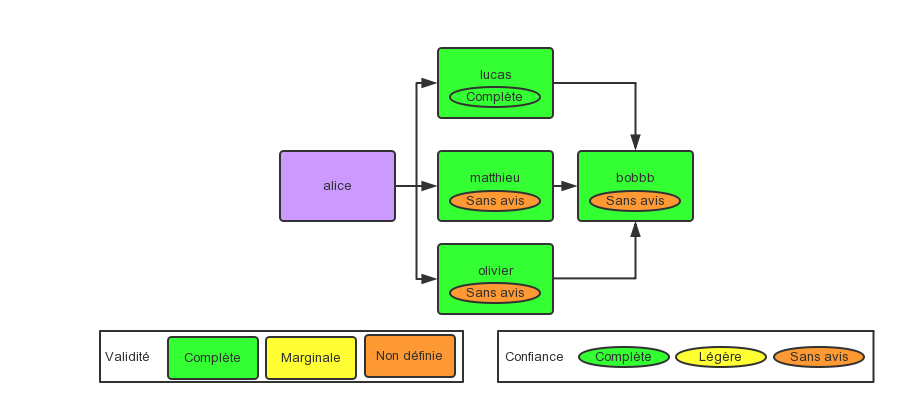
\includegraphics[scale=0.3]{tdcdemoComplete2.png}
\end{frame}

\subsection{OpenPGP}
\begin{frame}
    \frametitle{\color{white}OpenPGP}
    \begin{block}{Qu'est-ce que OpenPGP ?}
      \begin{itemize}
       \item Crée en 1997 par l'IETF (Internet Engineering Task Force)
       \item Protocol libre permettant de sécuriser l'échange d'email.
       \item Définit différents formats de paquets (message chiffré, signature, clef privée, clef publique...).
       \item Se base sur le logiciel PGP.
         \item Aujourd'hui normalisé dans la RFC 4880.
       \end{itemize} 
    \end{block}
\end{frame}

\subsection{GnuPG}
\begin{frame}
    \frametitle{\color{white}GnuPG}
    \begin{block}{Qu'est-ce que GnuPG ?}
      \begin{itemize}
        \item GNU Privacy Guard (GPG)
        \item Logiciel libre créé par Werner KOCH en 1997.
        \item Basé sur le standard OpenPGP.
        \item Alternative à PGP.
      \end{itemize}
    \end{block}
\end{frame}